TODO
In this chapter I will describe obtained results on each test machine. I will show scheduling executed and improvements on cache miss migration  ...

The scheduling that the developed patch should be perform is showed in fig TODO

TODO fig schedule

According to amdhal Law \cite{lcs}:
	
\begin{equation}
       Speedup = (\frac{P_{1}}{S_{1}} + \frac{P_{2}}{S_{2}} + ... \frac{P_{n}}{S_{n}})^{-1} 
\label{eq:amdhal}
\end{equation}

We will verify on each tested machine, if developed patch provide the expected speedup.

%%%%%%%%%%%%%%%%%%%%%%%%%%%%%%%%%%%%%%%%%%%%%%%%%%%%%%%%%%%%%%%%%%%%%%%%%%%%%
\section{Intel Xeon}

First of all, we check if the performed scheduled is what we exeptected. To do this, we use \textit{trace}

\begin{figure}[htbp]
\centering
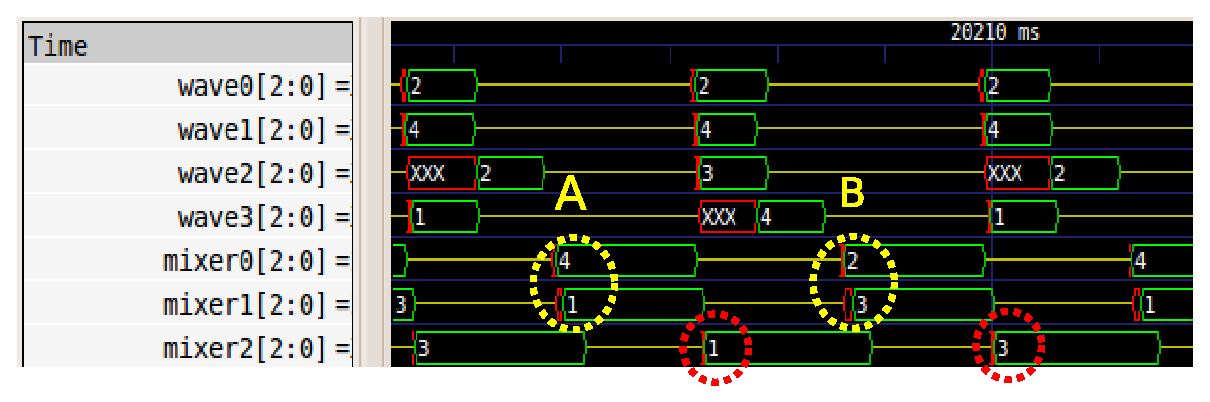
\includegraphics[width=\widefigure]{images/results_xeon/final_xeon.eps}
\caption{\figurecaption{trace TODO}}
\label{fig:trace_xeon}
\end{figure}

In Fig. \ref{fig:trace_xeon} we see that \textit{mixer2} can precede one of the waves and improve parallelism. We see that \textit{mixer0} chooses the best
cpu in term of temporal locality, for example: in step A \textit{mixer0} chooses CPU4 and not CPU2, because on CPU2 was executed \textit{wave2}, therefore 
L1 cache could be dirty, instead on CPU4 the last task executed is \textit{wave1}, therefore L1 cache should be clean. Also in step B, it is possible to 
note how \textit{mixer0} take care about the last task executed on CPU4 choosing CPU2.

%------------------------------------------------------------------------
\subsection{Cache misses}


\begin{figure}[htbp]
\centering
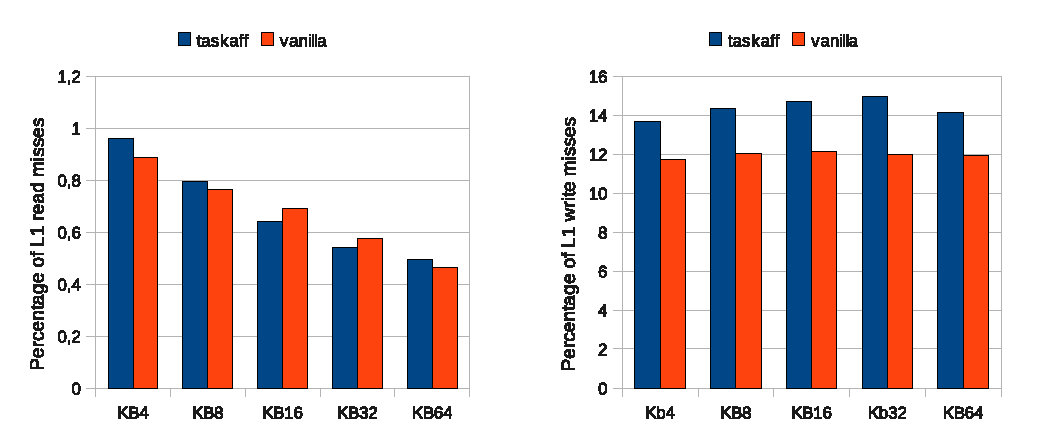
\includegraphics[width=\widefigure]{images/results_xeon/l1_load_store_xeon.eps}
\caption{\figurecaption{L1 Read and Write misses on Xeon}}
\label{fig:l1_load_store_xeon}
\end{figure}

\begin{figure}[htbp]
\centering
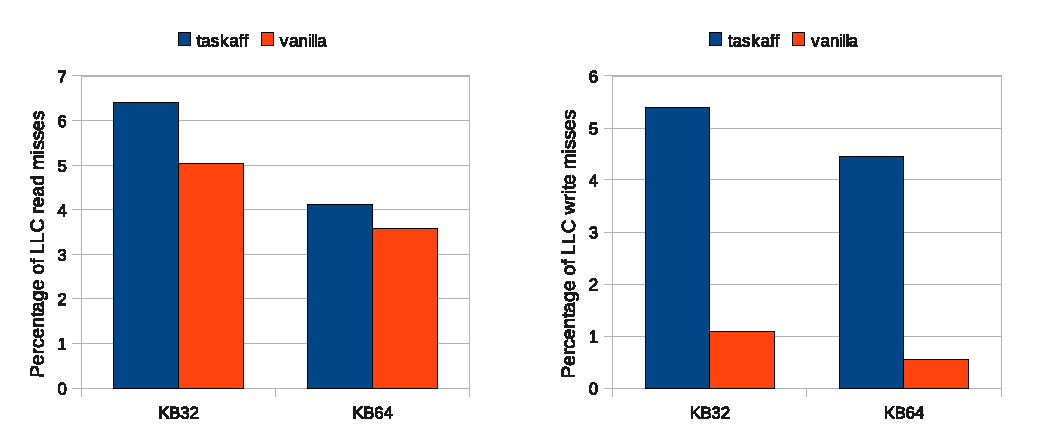
\includegraphics[width=\widefigure]{images/results_xeon/l2_load_store_xeon.eps}
\caption{\figurecaption{LLC Read and Write misses on Xeon}}
\label{fig:l2_load_store_xeon}
\end{figure}


%------------------------------------------------------------------------
\subsection{Performance}

\begin{figure}[htbp]
\centering
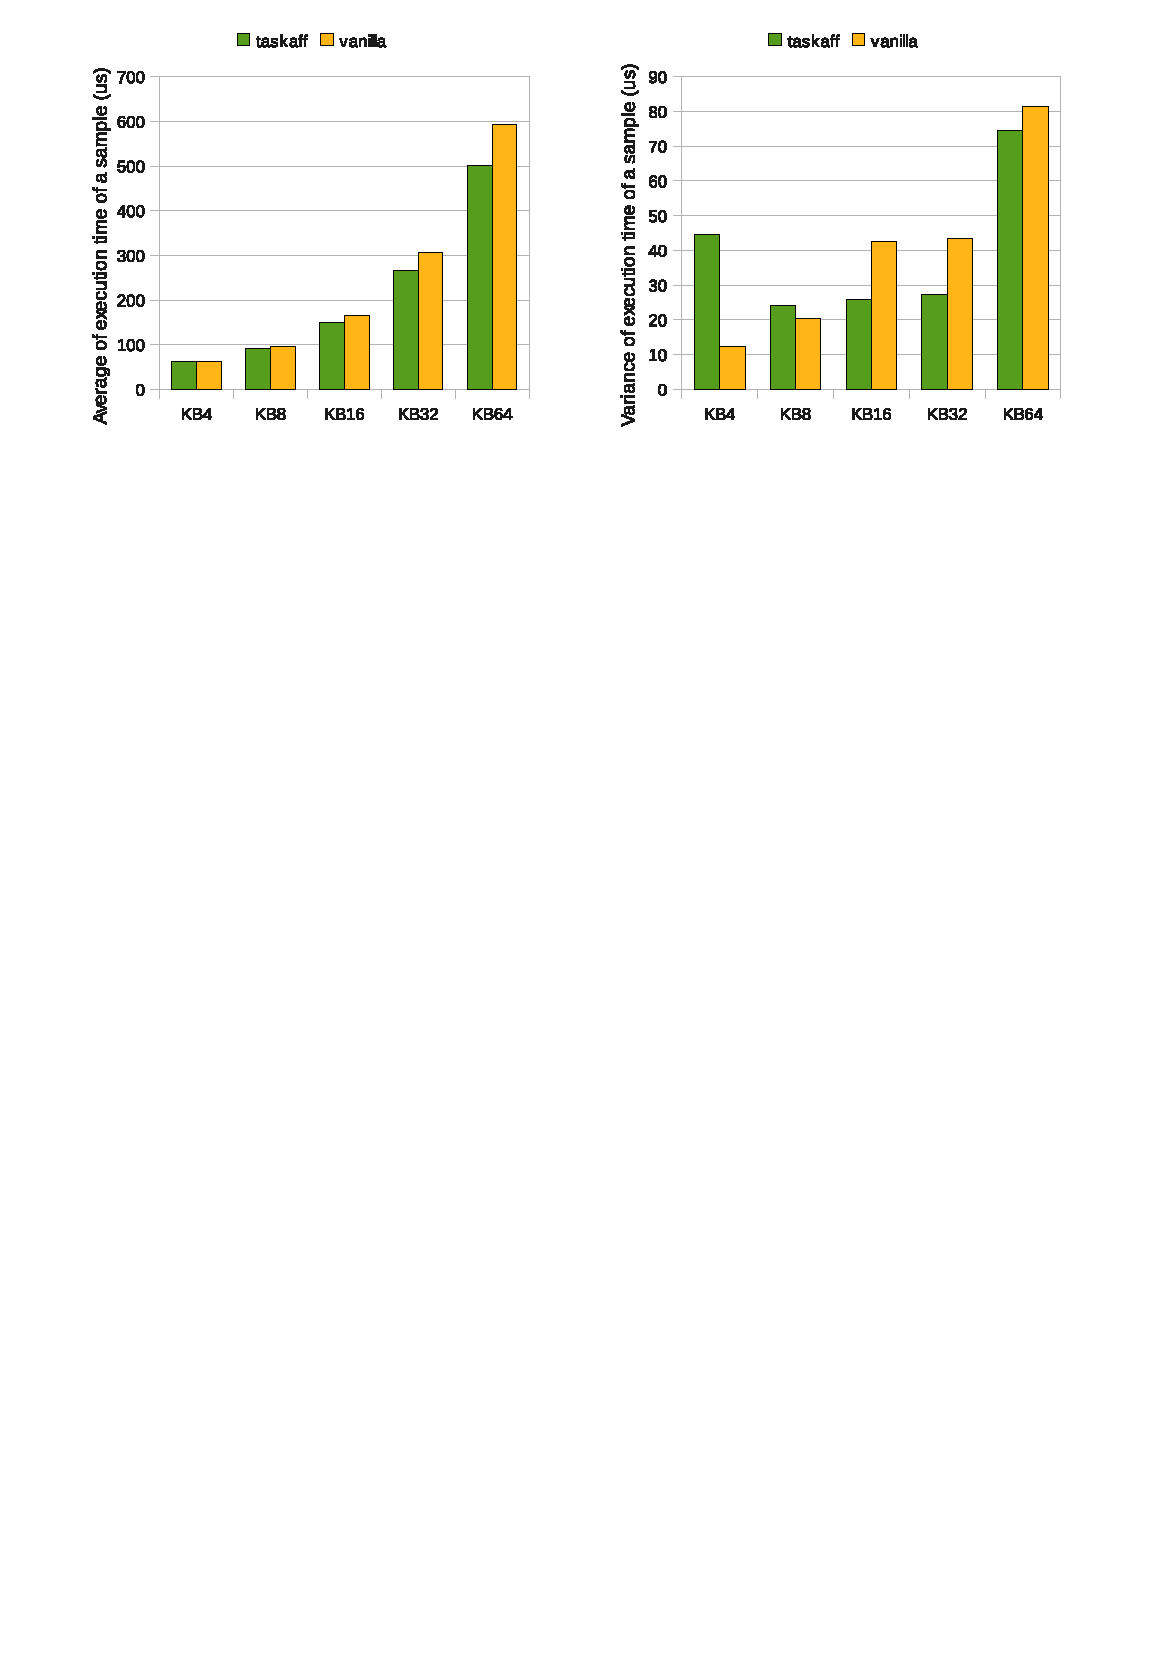
\includegraphics[width=\widefigure]{images/results_xeon/time_avg_var.eps}
\caption{\figurecaption{Average and Variance of execution time of a sample}}
\label{fig:time_avg_var_xeon}
\end{figure}
\newpage

%%%%%%%%%%%%%%%%%%%%%%%%%%%%%%%%%%%%%%%%%%%%%%%%%%%%%%%%%%%%%%%%%%%%%%%%%%%%%
\section{Intel i7}



%%%%%%%%%%%%%%%%%%%%%%%%%%%%%%%%%%%%%%%%%%%%%%%%%%%%%%%%%%%%%%%%%%%%%%%%%%%%%
\section{AMD}

TODO solo il trace dicendo che non funziona



